\paragraph{}Les fonctionnements des actions possibles au sein des applications étant sensiblement les mêmes, ceux ci seront décrits en utilisant deux diagrammes de séquence “type” afin d’éviter de créer une multitude de diagrammes redondants. Cependant, certains fonctionnements sont plus particuliers et seront donc expliqués via des diagrammes de séquence uniques.

    \begin{figure}[ht]
        \centering
        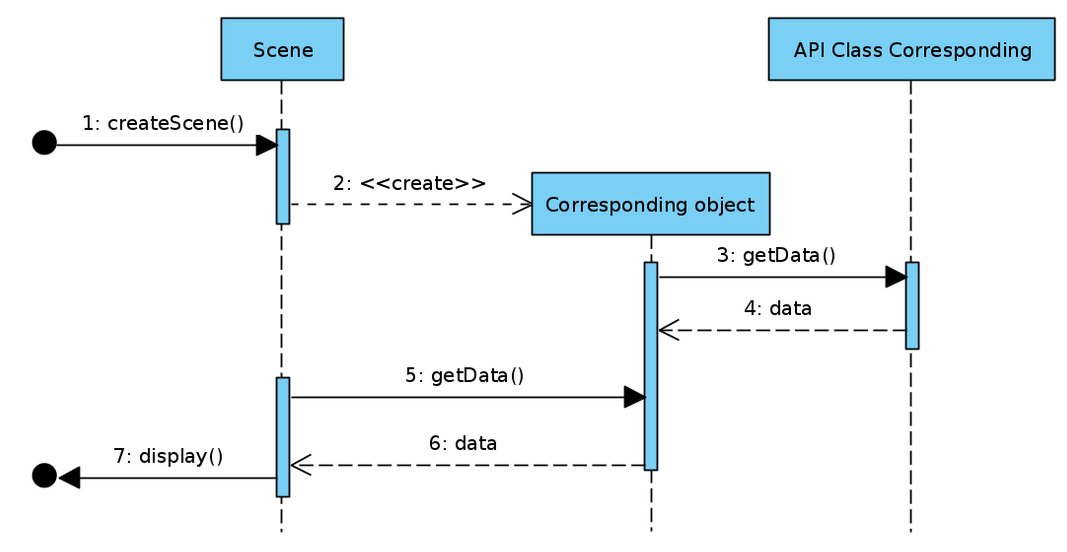
\includegraphics[scale=0.32]{img/type1.png}
        \caption{Diagramme de séquence du premier fonctionnement type}
        \label{fig1}
        \end{figure}

    \paragraph{}Le premier comportement type commence par la création d’une scene particulière(1). Cette scene va instancier un objet correspondant au contexte de la scene (2) (Si on est sur une fenêtre de compte en banque cela créera un objet Account). Cet objet va obtenir les données qui le caractérise via la base de donnée. Cela se fait via une méthode get() de la classe API correspondant à l’objet (3 et 4) (Par exemple, la classe Account utilisera la classe AccountController). Enfin l’objet peut être utilisé afin d’afficher des données sur une scene(5,6 et 7).

    \newpage

    \begin{figure}[ht]
        \centering
        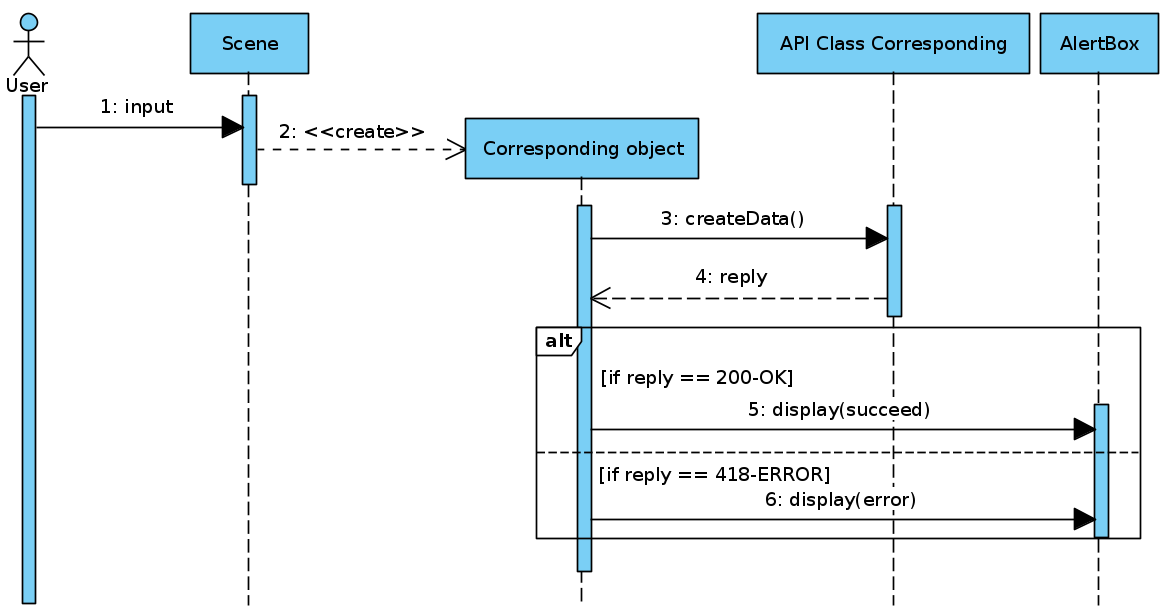
\includegraphics[scale=0.29]{img/type2.png}
        \caption{Diagramme de séquence du deuxième fonctionnement type}
        \label{fig2}
        \end{figure}

    \paragraph{}Le deuxième comportement type possible commence par une entrée de l’utilisateur via l’interface graphique via une scene particulière (1). Ces entrées vont permettre de créer un objet correspondant au contexte de la scene (2). Celui ci sera utilisé afin d’ajouter des données à la base de données via un appel create() sur la classe de l’API correspondant (3). Cet appel renverra une réponse (4), soit 200-OK si l’opération s’est bien déroulée, soit 418-ERROR si il y a eu une erreur ou que les données entrées sont déjà existantes. Selon la réponse, une petite fenêtre viendra signaler à l’utilisateur si l’opération s’est bien déroulée ou non (5 et 6).


    \newpage

    \begin{figure}[ht]
        \centering
        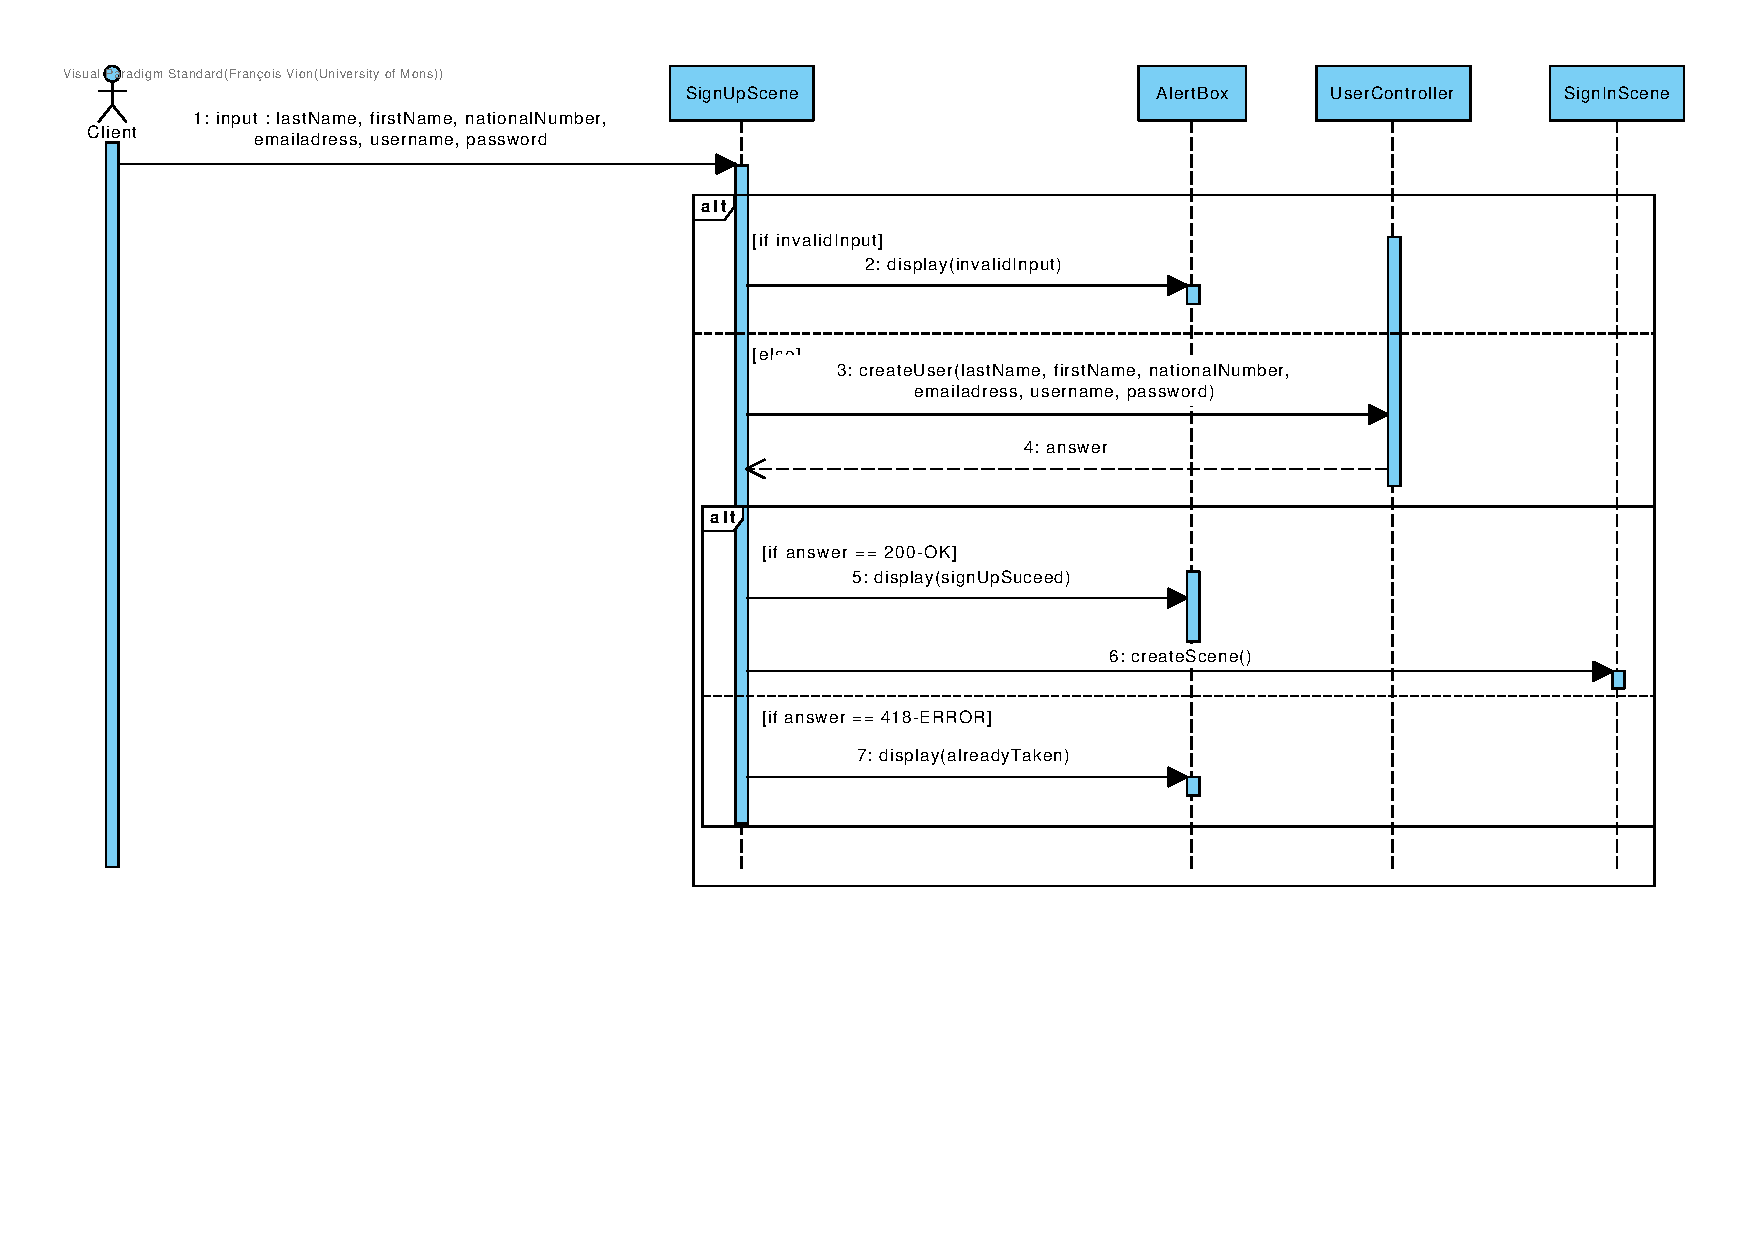
\includegraphics[scale=0.44]{img/createAccount.pdf}
        \caption{Diagramme de séquence de la création d'un compte}
        \label{fig3}
        \end{figure}

    \paragraph{} La création d’un compte se fait grâce à la scene SignUpScene qui prend comme entrée le nom, le prénom, le numéro de registre national, l’adresse email, un pseudonyme et un mot de passe (1). S’ils sont invalides, une fenêtre AlertBox est créée afin de le signaler à l’utilisateur (2). S’ils sont valides, la scene fait un appel createUser() à la classe d’API UserController (3), prenant en paramètre les inputs rentrés à l’étape (1). UserController renvoie une réponse à cet appel (4), à savoir 200-OK ou 418-ERROR, comme dans le premier fonctionnement. Si la réponse est 200-OK, une fenêtre affiche que l’opération est réussie (5) puis la scene suivante est chargée (6). Si la réponse est 418-ERROR, une fenêtre informe l’utilisateur que l’une de ses données est déjà utilisée (7).

    \newpage

    \begin{figure}[ht]
        \centering
        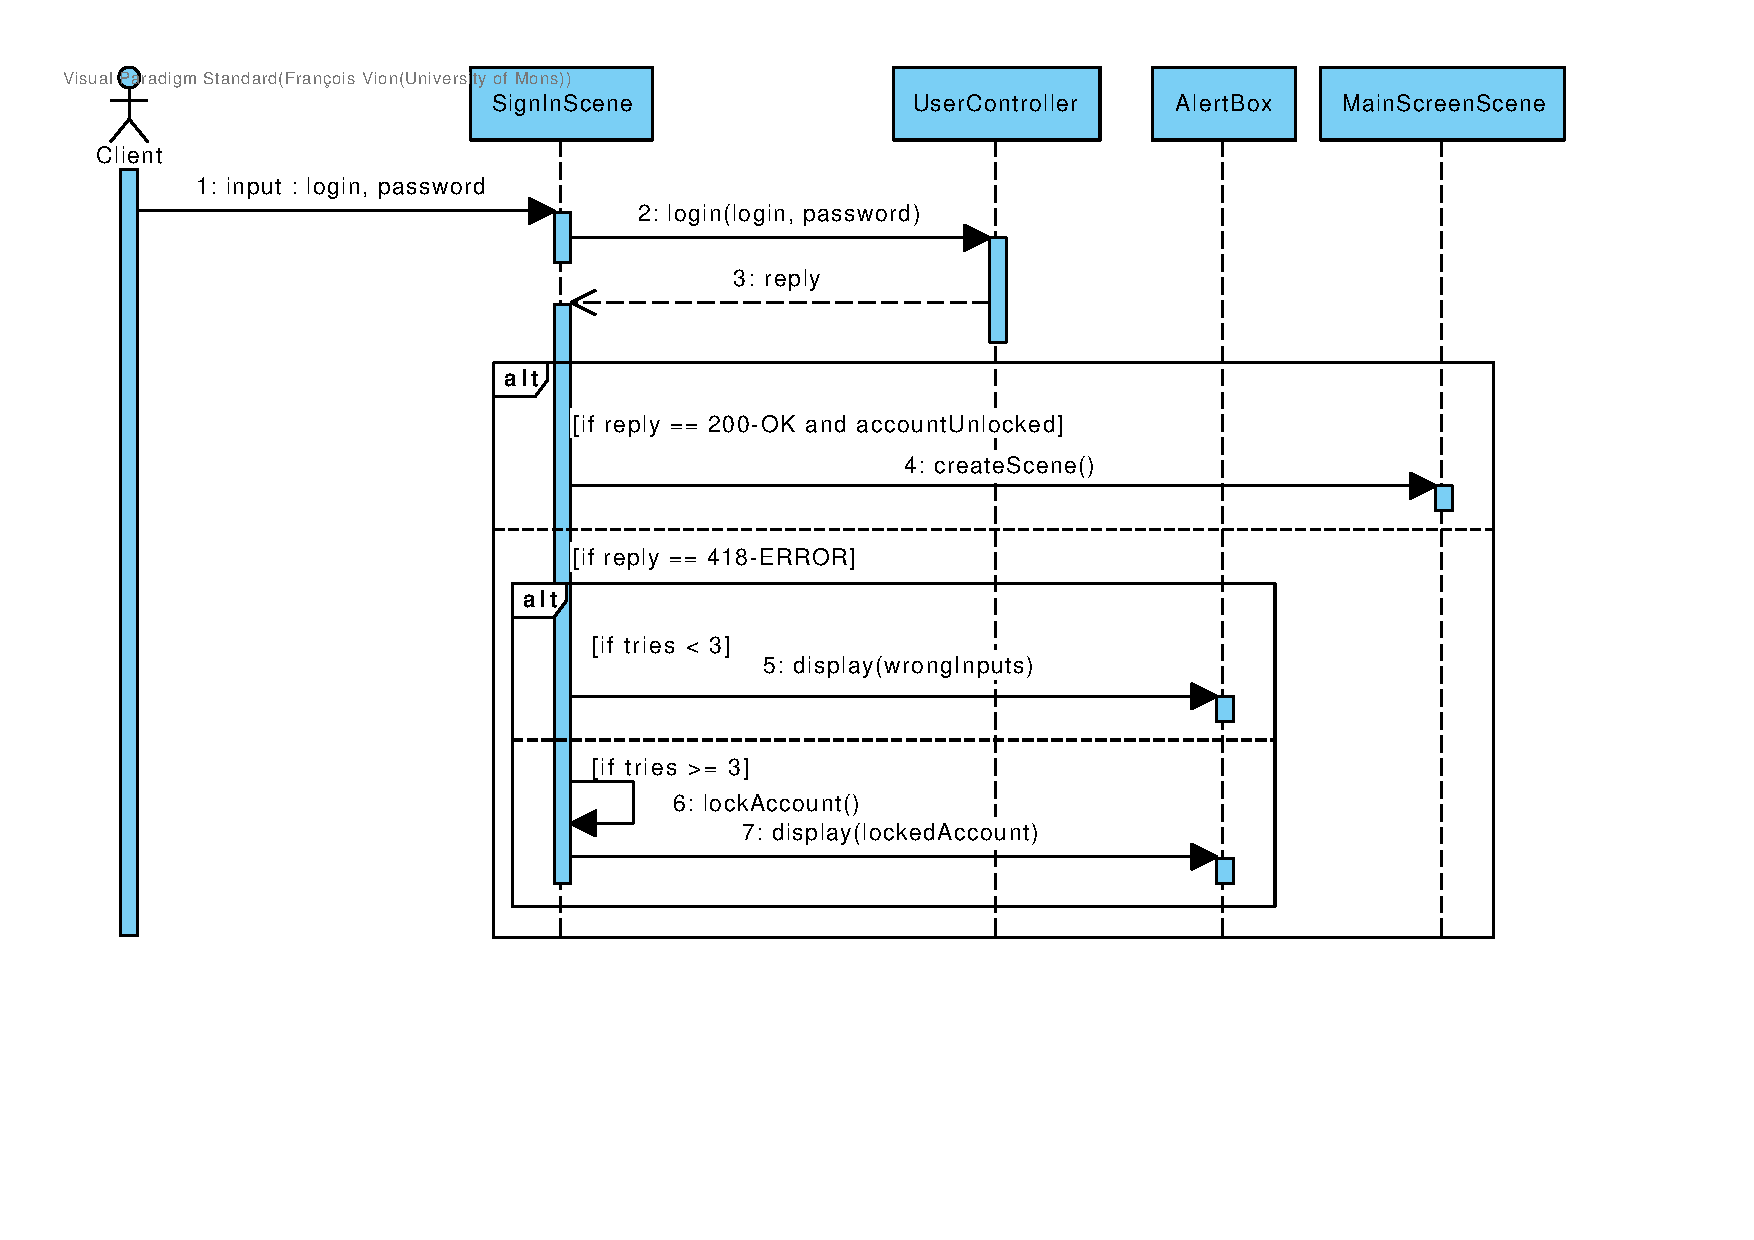
\includegraphics[scale=0.45]{img/Connexion.pdf}
        \caption{Diagramme de séquence de la création d'un compte}
        \label{fig4}
        \end{figure}

    \paragraph{} La connexion se fait grâce à la fenêtre SignInScene qui reçoit les entrées login et password de l’utilisateur (1). La scene va faire un appel login() à la classe d’API UserController avec comme paramètre les entrées de l’utilisateur (2). UserController va envoyer une réponse à la scene (3) avec 200-OK si l’identifiant et le mot de passe sont correct et 418-ERROR si ils sont incorrects. Si la réponse est 200-OK et que le compte n’est pas bloqué, la connexion sera réussie et la prochaine scene sera chargée (4). Si la réponse est 418-ERROR et que l’utilisateur a fait moins de 3 essais incorects, une fenêtre affichera que les entrées sont incorrectes grâce à la classe AlertBox (5). Si c’est le 3eme essai ou plus, le compte sera bloqué (6) et une fenêtre affichera que le compte est bloqué grâce à la classe AlertBox (7).
